\chapter{The Robot Models}
\label{cha:robots}

%Later: HOAP-2, NEC Papero (I already did a model in Blender), CITIZEN Eco-Be!, VisiON 4g (Fabio Dalla Libera is working on that), AIBO via RoSIML importer

The soccer simulation provides different robot models.
Below, we only describe the most advanced robot models that comes with the simulation package at this point in time. There are some other models which you can find in the directory \texttt{rcssserver3d/data/rsg/agent/}, e.g., the soccerplayer.rsg, or the hoap2.rsg files. These are currently not in use in any simulation, and considered experimental.

Besides that, work is in progress on other robot models and will be described here when usable. We plan to integrate an improved model of the HOAP-2 robot from Fujitsu Automation, and models of the VisiON 4g robot, and the Sony AIBO. For help on how to model new robots for your simulation, please have a look at tutorials in the SimSpark Wiki at \\

\url{http://simspark.sourceforge.net/wiki/}.





%-SECTION-----------------------------------------------------------
%---------------------------- Soccerbot ----------------------------
%-------------------------------------------------------------------
\section{Soccerbot}

The Soccerbot is a humanoid robot with 20 degrees of freedom (DOF) as depicted in figure \ref{fig:soccerbotdof}. Its current dimensions are quite unrealistic for a real humanoid robot (see table \ref{table:dimensions}) which is due to instabilities in the physics simulation at the time the robot was first modeled. This is a serious shortcoming of this robot model and should be changed. Another open issue is that the joint ranges are not limited in the current model. This allows for very unrealistic movements which can be fun to watch, but can lead to unfair behavior in a competition.

\begin{figure}[htp]
\begin{minipage}[b]{0.5\linewidth} 
\centering
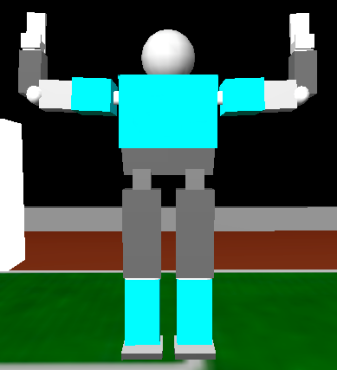
\includegraphics[width=6cm]{fig/soccerbotfront}
\caption{Frontal view of the Soccerbot in the simulation}
\end{minipage}
\hspace{0.5cm}
\begin{minipage}[b]{0.5\linewidth}
\centering
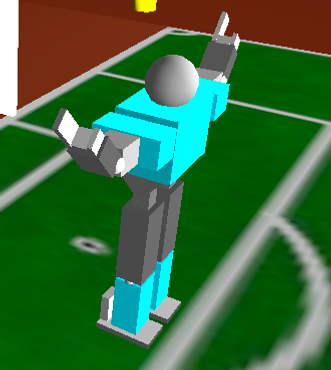
\includegraphics[width=6cm]{fig/soccerbotside}
\caption{Side view of the Soccerbot in the simulation}
\end{minipage}
\end{figure}



%-SUB-SECTION-------------------------------------------------------
%--------------------------- Equipment -----------------------------
%-------------------------------------------------------------------
\subsection{Equipment \& Parameter}
The Soccerbot has several kinds of sensors available. It uses a
(omni-directional) vision sensor (see section \ref{sec:visionperceptor}) to get
information about objects in its environment\footnote{It is currently located in
the center of the torso, which should be changed to be in the head.}. In order
to detect the contact with the ground and the resulting force at the feet, it is
equipped with a Force Resistance Perceptor (see section \ref{sec:FRP}) in each
foot. It can sense the current simulation time with a GameState Perceptor (see
section \ref{sec:gamestateperceptor}) and the change in orientation of its torso
with a GyroRate Perceptor (see section \ref{sec:GYR}). Furthermore, it has
proprioceptive sensors that allow to sense the angle of each joint (see sections
\ref{sec:HJP} and \ref{sec:UJP} for HingeJoint Perceptor and UniversalJoint
Perceptor descriptions, respectively). An overview over the joint perceptors and
effectors is given in table \ref{table:perceptorNames}.

\begin{figure}[htp]
  \centering
  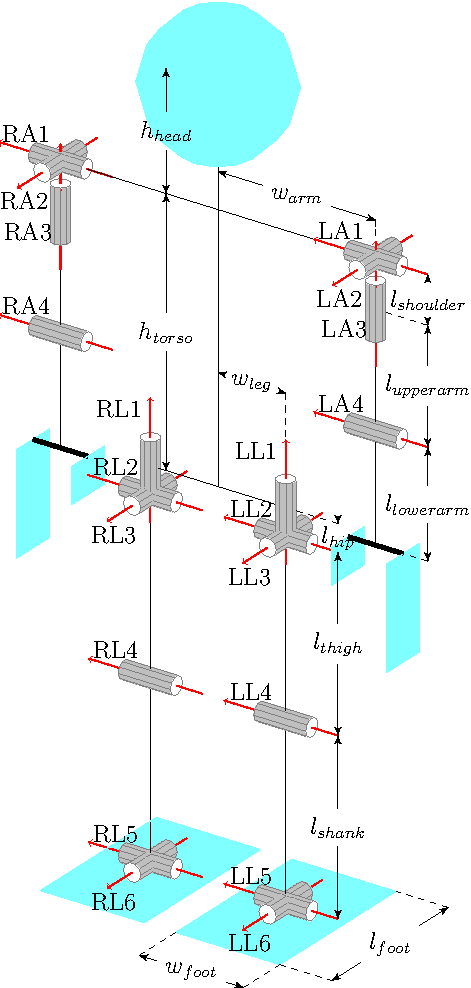
\includegraphics[height=0.6\textwidth]{fig/soccerbot056}
  \caption{Overview of the degrees of freedom of the Soccerbot}
  \label{fig:soccerbotdof}
\end{figure}

\begin{table}
\caption{Perceptor and effector names}
\label{table:perceptorNames}
\begin{center}
\begin{tabular}{|l|l|l|l|}
\hline
{\bf Connection between}  & {\bf Joint type} & {\bf Perceptor name}& {\bf
Effector name} \\
\hline\hline
Shoulder - body  & Universal joint & laj1\_2  raj1\_2 & lae1\_2   rae1\_2 \\
\hline
Upper arm - shoulder  & Hinge joint & laj3  raj3 & lae3   rae3 \\
\hline
Forearm - upper arm  & Hinge joint & laj4  raj4 & lae4   rae4 \\
\hline
Hip - body  & Hinge joint & llj1  rlj1 & lle1   rle1 \\
\hline
Upper leg - hip & Universal joint & llj2\_3  rlj2\_3 & lle2\_3   rle2\_3 \\
\hline
Lower leg - upper leg & Hinge joint & llj4  rlj4 & lle4   rle4 \\
\hline
foot - lower leg & Universal joint & llj5\_6  rlj5\_6 & lle5\_6   rle5\_6 \\
\hline
\end{tabular}
\end{center}
\end{table}

Figure \ref{fig:examplemsg} shows an example message which the agent receives
from the server in a single simulation cycle including sense information from
all the perceptors of the agent.

The measurements of all body parts of the Soccerbot are listed in table
\ref{table:dimensions}.

\begin{figure}[h!]
 \centering
\lstset{language=SSML}
\begin{lstlisting}
(time (now 19.60))
(GYR (n torso) (rt -0.02 -0.01 -0.00))
(See
    (F1L (pol 10.34 45.02 -16.70))
    (F2L (pol 68.43 174.14 -2.56))
    (F1R (pol 103.28 -86.10 -1.66))
    (F2R (pol 123.46 -123.42 -1.43))
    (G1L (pol 27.94 165.40 -6.96))
    (G2L (pol 35.03 168.43 -5.56))
    (G1R (pol 106.49 -104.59 -1.83))
    (G2R (pol 108.57 -108.33 -1.80))
    (B (pol 56.95 -122.42 -3.02))
    (P (team teamRed) (id 2) (pol 10.50 -179.98 -0.07)))
(UJ (n laj1_2) (ax1 0.00) (ax2 90.63))
(UJ (n raj1_2) (ax1 -0.00) (ax2 90.63))
(HJ (n laj3) (ax 90.77))
(HJ (n raj3) (ax -90.77))
(HJ (n laj4) (ax 87.96))
(HJ (n raj4) (ax 88.40))
(HJ (n llj1) (ax 0.03))
(HJ (n rlj1) (ax -0.02))
(UJ (n llj2_3) (ax1 -0.03) (ax2 0.02))
(UJ (n rlj2_3) (ax1 -0.02) (ax2 0.01))
(HJ (n llj4) (ax 0.05))
(HJ (n rlj4) (ax 0.04))
(TCH (n lf) (val 1))
(UJ (n llj5_6) (ax1 0.05) (ax2 -0.01))
(TCH (n rf) (val 1))
(UJ (n rlj5_6) (ax1 0.04) (ax2 -0.00))
\end{lstlisting}
 \caption{An example message from the server to the Soccerbot including information from all the sensors.}
 \label{fig:examplemsg}
\end{figure}


\begin{table}
\centering
\begin{tabular}[htbp]{|l|c|c|c|c|}
  \hline
  {\bf Name} & {\bf Width} & {\bf Depth} & {\bf Height} & {\bf Mass} \\
  \hline\hline
  head & \multicolumn{3}{|c|}{0.39m (radius)} & 0.3kg\\ \hline
  torso & 1.37m & 0.96m & 1.41m & 1.8kg \\ \hline
  left\_shoulder & 0.445m & 1.017m & 0.536m & 0.5kg \\ \hline
  right\_shoulder & 0.445m & 1.017m & 0.536m & 0.5kg \\ \hline
  left\_upper\_arm & 0.445m & 0.398m & 0.506m & 0.2kg \\ \hline
  right\_upper\_arm & 0.445m & 0.398m & 0.506m & 0.2kg \\ \hline
  left\_lower\_arm & 0.445m & 0.316m & 0.6m & 0.2kg \\ \hline
  left\_lower\_arm & 0.445m & 0.316m & 0.6m & 0.2kg \\ \hline
  left\_hip & 0.273m & 0.273m & 0.2m & 0.1kg \\ \hline
  right\_hip & 0.273m & 0.273m & 0.2m & 0.1kg \\ \hline
  left\_thigh & 0.56m & 0.56m & 1.3m & 0.25kg \\ \hline
  right\_thigh & 0.56m & 0.56m & 1.3m & 0.25kg \\ \hline
  left\_shank & 0.56m & 0.56m & 0.964m & 0.25kg \\ \hline
  right\_shank & 0.56m & 0.56m & 0.964m & 0.25kg \\ \hline
  left\_foot & 0.6m & 0.956m & 0.095m & 0.1kg \\ \hline
  right\_foot & 0.6m & 0.956m & 0.095m & 0.1kg \\
  \hline
\end{tabular}
\caption{Physical properties of the Soccerbot.}
\label{table:dimensions}
\end{table}





%-SECTION-----------------------------------------------------------
%------------------------------- Nao -------------------------------
%-------------------------------------------------------------------
\section{Nao}
\label{sec:nao}
The Nao humanoid robot manufactured by Aldebaran Robotics. This is the robot
currently used in the competitions of the 3D Soccer Simulation League at
RoboCup. Its height is about $57cm$ and its weight is around $4.5kg$. Its biped
architecture with 22 degrees of freedom allows Nao to have great mobility. The
rcssserver3D can simulate the Nao robot nicely, see \autoref{fig:nao}.
\begin{figure}[htp]
  \centering
  \def\mheight{5cm}
  \subfigure[real robot]{
    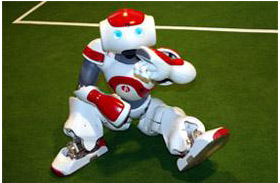
\includegraphics[height=\mheight]{fig/realNao}
  }
  \subfigure[virtual robot]{
    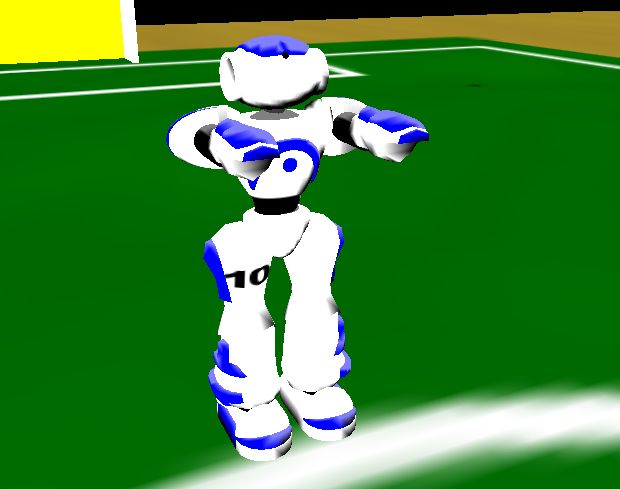
\includegraphics[height=\mheight]{fig/virtualNao}
  }
  \caption{The Nao humanoid robot.}
  \label{fig:nao}
\end{figure}
\pagebreak



%-SUB-SECTION-------------------------------------------------------
%--------------------------- Equipment -----------------------------
%-------------------------------------------------------------------
\subsection{Equipment}
This section is quite important to the agent development for the specific
perceptors and effectors used to represent this robot.
The Nao robot model is equipped with a powerful selection of the perceptors and
effectors described in chapter \ref{cha:simspark}, to provide a widespread
information base for agent development.

The Nao robot possess a gyroscope and a accelerometer, to keep track of radial
as well as axial movement of itself in the three dimensional space.
Both of them are located in the center of the torso, therefore the only
available identifier to this two perceptors is ``\texttt{torso}''.
  
In order to detect the contact with the ground and other objects in the
simulation, one force resistance perceptor in each foot indicates the actual
pressure on it. Possible identifiers are ``\texttt{lf}'' and ``\texttt{rf}'',
for the left and right foot.

To get information about different objects in its environment the Nao robot
possess a restricted vision perceptor in the center of its head.
Note: The visual perception is described in a right hand system facing the
x-axis.

For communication purposes it is equipped with a say effector and the
corresponding hear perceptor.

The position of each joint is represented by a hinge joint perceptor and
manipulable through the corresponding hinge joint effector. For a complete
list of all available joints of the Nao robot and their corresponding
identifiers please refer to table \ref{table:naojoints}. The arrangement of the
joints and their relative orientation is shown in figure \ref{fig:naojoints}.

The gamestate perceptor is used to inform about the actual play time and play
mode.

Figure \ref{fig:nao_examplemsg} shows an example message which the agent
receives from the server in a single simulation cycle including sense
information from all the perceptors of the agent.

\begin{table}[htbp]
\centering
\begin{tabular}[htbp]{|r|l|c|c|c|}
  \hline
  {\bf No.} & {\bf Description} & {\bf Hinge Joint} & {\bf Perceptor name} &
  {\bf Effector name} \\ \hline\hline
  1 & Neck Yaw & [0][0] & \texttt{hj1} & \texttt{he1} \\ \hline
  2 & Neck Pitch & [0][1] & \texttt{hj2} & \texttt{he2} \\ \hline
  3 & Left Shoulder Pitch & [1][0] & \texttt{laj1} & \texttt{lae1} \\ \hline
  4 & Left Shoulder Yaw & [1][1] & \texttt{laj2} & \texttt{lae2} \\ \hline
  5 & Left Shoulder Roll & [1][2] & \texttt{laj3} & \texttt{lae3} \\ \hline
  6 & Left Arm Yaw & [1][3] & \texttt{laj4} & \texttt{lae4} \\ \hline
  7 & Left Hip YawPitch & [2][0] & \texttt{llj1} & \texttt{lle1} \\ \hline
  8 & Left Hip Roll & [2][1] & \texttt{llj2} & \texttt{lle2} \\ \hline
  9 & Left Hip Pitch & [2][2] & \texttt{llj3} & \texttt{lle3} \\ \hline
  10 & Left Knee Pitch & [2][3] & \texttt{llj4} & \texttt{lle4} \\ \hline
  11 & Left Foot Pitch & [2][4] & \texttt{llj5} & \texttt{lle5} \\ \hline
  12 & Left Foot Roll & [2][5] & \texttt{llj6} & \texttt{lle6} \\ \hline
  13 & Right Hip YawPitch & [3][0] & \texttt{rlj1} & \texttt{rle1} \\ \hline
  14 & Right Hip Roll & [3][1] & \texttt{rlj2} & \texttt{rle2} \\ \hline
  15 & Right Hip Pitch & [3][2] & \texttt{rlj3} & \texttt{rle3} \\ \hline
  16 & Right Knee Pitch & [3][3] & \texttt{rlj4} & \texttt{rle4} \\ \hline
  17 & Right Foot Pitch & [3][4] & \texttt{rlj5} & \texttt{rle5} \\ \hline
  18 & Right Foot Roll & [3][5] & \texttt{rlj6} & \texttt{rle6} \\ \hline
  19 & Right Shoulder Pitch & [4][0] & \texttt{raj1} & \texttt{rae1} \\ \hline
  20 & Right Shoulder Yaw & [4][1] & \texttt{raj2} & \texttt{rae2} \\ \hline
  21 & Right Shoulder Roll & [4][2] & \texttt{raj3} & \texttt{rae3} \\ \hline
  22 & Right Arm Yaw & [4][3] & \texttt{raj4} & \texttt{rae4} \\
  \hline
\end{tabular}
\caption{Available hinge joints of Nao robot.}
\label{table:naojoints}
\end{table}%


\begin{figure}[htbp]
  \centering
  \includegraphics[width=\textwidth]{fig/nao_joints_DH}
  \caption{The joints of Nao robot.}
  \label{fig:naojoints}
\end{figure}


\begin{figure}[htbp]
 \centering
\lstset{language=SSML}
\begin{lstlisting}
(time (now 93.60)) 
(GS (t 0.00) (pm BeforeKickOff))
(hear 0.00 self 1000-501)
(GYR (n torso) (rt -0.35 -0.36 -0.01))
(ACC (n torso) (a 0.20 -0.20 9.79))
(HJ (n hj1) (ax 0.33))
(HJ (n hj2) (ax -3.31))
(See 
    (G2R (pol 17.55 -3.33 4.31)) 
    (G1R (pol 17.52 3.27 4.07))
    (F1R (pol 18.52 18.94 1.54))
    (F2R (pol 18.52 -18.91 1.52))
    (B (pol 8.51 -0.21 -0.17))
    (P (team teamRed) (id 1)
        (head (pol 16.98 -0.21 3.19))
        (rlowerarm (pol 16.83 -0.06 2.80))
        (llowerarm (pol 16.86 -0.36 3.10))
        (rfoot (pol 17.00 0.29 1.68))
        (lfoot (pol 16.95 -0.51 1.32)))
    (P (team teamBlue) (id 1) 
        (rlowerarm (pol 0.18 -33.55 -20.16))
        (llowerarm (pol 0.18 34.29 -19.80))))
(HJ (n raj1) (ax 31.72))
(HJ (n raj2) (ax -20.12))
(HJ (n raj3) (ax -0.01))
(HJ (n raj4) (ax 40.04))
(HJ (n laj1) (ax 64.37))
(HJ (n laj2) (ax 19.96))
(HJ (n laj3) (ax 0.09))
(HJ (n laj4) (ax -40.11))
(HJ (n rlj1) (ax -0.06))
(HJ (n rlj2) (ax 20.31))
(HJ (n rlj3) (ax -39.24))
(HJ (n rlj4) (ax 20.02))
(HJ (n rlj5) (ax 0.04))
(FRP (n rf) (c 0.01 -0.01 -0.02) (f -0.21 0.21 19.77))
(HJ (n rlj6) (ax 0.21))
(HJ (n llj1) (ax -0.01))
(HJ (n llj2) (ax 0.00))
(HJ (n llj3) (ax 19.70))
(HJ (n llj4) (ax -41.02))
(HJ (n llj5) (ax 20.31))
(FRP (n lf) (c 0.01 -0.01 -0.02) (f -0.21 0.20 25.45))
(HJ (n llj6) (ax -0.16))
\end{lstlisting}
 \caption{An example message from the server to the Nao robot including information from all the sensors.}
 \label{fig:nao_examplemsg}
\end{figure}



%-SUB-SECTION-------------------------------------------------------
%--------------------------- Parameters ----------------------------
%-------------------------------------------------------------------
\subsection{Parameters}
Beside the perceptors and effectors it's also quite important to the agent
development to be aware of the parameters used to construct the robot. This
section gives information about body measurements and the arrangement of the
different body parts. While the box model of the Nao robot is shown in figure
\ref{fig:nao_boxmodel}, a detailed description of the Nao configuration is given
in table\,\ref{tab:nao-conf}.

\begin{figure}[b!]
  \centering
    \includegraphics[width=\textwidth]{fig/nao_boxmodel}
  \caption{The Nao's boxmodel.}
  \label{fig:nao_boxmodel}
\end{figure}

\begin{landscape}
\begin{table}
  \centering
  \caption{Configuration of Nao (see the text for the meaning of each
    column).}
  \label{tab:nao-conf}
  \newcommand{\threegrid}[1]{\multicolumn{3}{c|}{#1}}
  \newcommand{\fourgrid}[1]{\multicolumn{4}{c|}{#1}}
  \begin{tabular}{|l|l|r@{,}r@{,}r@{}c|l|l|c|r@{,}r@{,}r|r@{,}r@{,}l@{}c|l|l|}
    \hline
    \multicolumn{8}{|c|}{\bf Body part} & \multicolumn{10}{c|}{\bf Hinge joint}\\
    \hline
    {\bf Name} & {\bf Parent} & \fourgrid{\bf Translation} & {\bf Mass} & {\bf Geometry} & {\bf Name} & \threegrid{\bf Anchor} & \fourgrid{\bf Axis} & {\bf Min} & {\bf Max}\\
    \hline\hline
    neck & torso & $0$&$0$&$0.09$& & $0.05$ & Cylinder & \texttt{hj1} & $0$&$0$&$0$ & $0$&$0$&$1$& & $-120$ & $120$\\
    & & \fourgrid{} & & L: $0.08$ R: $0.015$ & & \threegrid{} & \fourgrid{} & &\\
    \hline
    head & neck & $0$&$0$&$0.065$& & $0.35$ & Sphere $0.065$ & \texttt{hj2} & $0$&$0$&$-0.005$ & $1$&$0$&$0$& & $-45$ & $45$\\
    \hline
    shoulder & torso & $0.098$&$0$&$0.075$&(r)  & $0.07$ & Sphere $0.01$& \texttt{raj1} & $0$&$0$&$0$ & $1$&$0$&$0$& & $-120$ & $120$\\
    & & $-0.098$&$0$&$0.075$&(l) & & & \texttt{laj1} & \threegrid{} & \fourgrid{} & & \\
    \hline
    upperarm & shoulder & $0.01$&$0.02$&$0$&(r) & $0.150$ & Box & \texttt{raj2} & \threegrid{-Translation} & $0$&$0$&$1$& & $-95$(r) & $1$(r)  \\
    & & $-0.01$&$0.02$&$0$&(l) & & $0.07$, $0.08$, $0.06$ & \texttt{laj2} & \threegrid{} & \fourgrid{} & $-1$(l) & $95$(l) \\
    \hline
    elbow & upperarm & $-0.01$&$0.07$&$0.009$&(r) & $0.035$ & Sphere $0.01$ & \texttt{raj3} & $0$&$0$&$0$ & $0$&$1$&$0$& & $-120$ & $120$ \\
    & & $0.01$&$0.07$&$0.009$&(l) & & & \texttt{laj3} & \threegrid{} & \fourgrid{} & &\\
    \hline
    lowerarm & elbow & $0$&$0.05$&$0$& & $0.2$ & Box & \texttt{raj4} & \threegrid{-Translation} & $0$&$0$&$1$& & $-1$(r) & $90$(r) \\
    & & \fourgrid{} & & $0.05$, $0.11$, $0.05$ & \texttt{laj4} & \threegrid{} & \fourgrid{} & $-90$(l) & $1$(l) \\
    \hline
    hip1 & torso & $0.055$&$-0.01$&$-0.115$&(r) & $0.09$ & Sphere $0.01$ & \texttt{rlj1} & $0$&$0$&$0$ & $-0.7071$&$0$&$0.7071$&(r)  & $-90$ & $1$ \\
     & & $-0.055$&$-0.01$&$-0.115$&(l) & & & \texttt{llj1} & \threegrid{} & $-0.7071$&$0$&$-0.7071$&(l) & &\\
    \hline
    hip2 & hip1 & $0$&$0$&$0$& & $0.125$ & Sphere $0.01$ & \texttt{rlj2} & $0$&$0$&$0$ & $0$&$1$&$0$& & $-45$(r) & $25$(r)\\
    & & \fourgrid{} & & & \texttt{llj2} & \threegrid{} & \fourgrid{} & $-25$(l) & $45$(l) \\
    \hline
    thigh & hip2 & $0$&$0.01$&$-0.04$& & $0.275$ & Box & \texttt{rlj3} & \threegrid{-Translation} & $1$&$0$&$0$& &  $-25$ & $100$\\
    & & \fourgrid{} & & $0.07$, $0.07$, $0.14$ & \texttt{llj3} & \threegrid{} & \fourgrid{} & & \\
    \hline
    shank & thigh & $0$&$0.005$&$-0.125$& & $0.225$ & Box  & \texttt{rlj4} & $0$&$-0.01$&$0.045$ & $1$&$0$&$0$& & $-130$ & $1$\\
    & & \fourgrid{} & & $0.08$, $0.07$, $0.11$ & \texttt{llj4} & \threegrid{} & \fourgrid{} & &\\
    \hline
    ankle & shank & $0$&$-0.01$&$-0.055$& & $0.125$ & Sphere $0.01$ & \texttt{rlj5} & $0$&$0$&$0$ & $1$&$0$&$0$& & $-45$ & $75$\\
    & & \fourgrid{} & & & \texttt{llj5} & \threegrid{} & \fourgrid{} & &\\
    \hline
    foot & ankle & $0$&$0.03$&$-0.035$& & $0.2$ & Box & \texttt{rlj6} & $0$&$-0.03$&$0.035$ & $0$&$1$&$0$& & $-25$(r) & $45$(r)\\
    & & \fourgrid{} & & $0.08$, $0.16$, $0.03$ & \texttt{llj6} & \threegrid{} & \fourgrid{} & $-45$(l) & $25$(l)\\
    \hline
    torso &  & \fourgrid{} & $1.2171$ & Box & & \threegrid{} & \fourgrid{} & &\\
    & & \fourgrid{} & & $0.1$, $0.1$, $0.18$ & & \threegrid{} & \fourgrid{} & &\\
    \hline
  \end{tabular}
\end{table}
\end{landscape}
Meaning of each column from left to right in \ref{tab:nao-conf}
are explained as follow:
\begin{description}
\item[Name] the body part name of Nao
\item[Parent]  the parent of the body
\item[Translation] the offset relative to its parent (meter)
\item[Mass] the mass of this body (kilogram)
\item[Geometry] the size of its geometry representation (meter)
\item[Name] the joint name installed on this body
\item[Anchor] the offset of the joint anchor relative to the body that
  installed on (meter)
\item[Axis] the joint axis relative to the body that installed on (pitch, roll,
yaw)
\item[Min] the min angle that the joint can reach (degrees)
\item[Max] the max angle that the joint can reach (degrees)
\end{description}



%-SUB-SECTION-------------------------------------------------------
%------------------------- Implementation --------------------------
%-------------------------------------------------------------------
\subsection{Implementation}
The Nao robot model is implemented in the rsg files under
\texttt{rcssserver3d/data/rsg/agent/nao}, see \autoref{tab:nao-implement}
for details. This section goes much deeper and is a little boring.
\begin{table}[htp]
  \centering
  \caption{The rsg files of Nao robot}
  \label{tab:nao-implement}
  \begin{tabular}{lp{0.6\textwidth}}
    \hline
    {\bf File Name}             & {\bf Description} \\
    \hline
    box\_appearance.rsg         & Install a box which is for the GL
    render. \\
    box\_physics.rsg            & Install a box that has physics
    effect(ODE related) \\
    box\_physics\_nocollider.rsg & Install a box that only has dynamics
    effect (mass, linear velocity, etc). But it can never collide to
    the others. \\
    box\_physics\_with\_handler.rsg & Not only do the job as file
    “box\_physics.rsg”, but also install a touchperceptorhandler under
    the BoxCollider Node. \\
    capsule\_appearance.rsg   & Install a capsule which is
    for the GL render. \\
    capsule\_physics.rsg      & Install a capsule that has
    physics effect(ODE related) \\
    capsule\_physics\_nocollider.rsg & Install a capsule that
    only has dynamics effect (mass, linear velocity, etc). But it can
    never collide to the others. \\
    contactjointhandler.rsg    & Install a contactjointhandler to
    handle the collisions. \\
    dragcontroller.rsg         & Install a DragController. \\
    goal.rsg                   & Install the goal. \\
    hingejoint.rsg             & Install a hingejoint. \\
    \hline
  \end{tabular}
\end{table}

%%% Local Variables: 
%%% mode: latex
%%% TeX-master: "user-manual"
%%% End: 
